\chapter{Elektrizität und Magnetismus als ein relativistisches Feld}

Wir haben untersucht, wie sich ein geladenes Teilchen in einem vorgegebenen elektromagnetischen Feld bewegt. Die noch offene Hälfte des Problems betrifft das Feld selbst: wie sich elektrische und magnetische Felder entwickeln und wie Ladung und Strom als ihre Quellen wirken. Diese Fragen beantworten die Maxwell-Gleichungen. Bevor wir sie hinschreiben, lohnt es sich jedoch, das physikalische Rätsel wieder aufzugreifen, das ihre relativistische Struktur unausweichlich machte.

Dies ist ein bewusster Rückzug vom Formalismus. Das Wirkungsprinzip kommt später wieder zur Sprache. Der Grund für diesen anderen Ausgangspunkt ist, dass wir zunächst sehen wollen, warum elektrische und magnetische Felder Bestandteile eines einzigen Objekts sein müssen, bevor wir ihre Dynamik aus einer Wirkung herleiten.

\section{Das Rätsel im ersten Absatz von Einstein}

Während eines Besuchs in Belgien führte ein Gespräch über die frühen Solvay-Konferenzen zurück zu Einsteins 1905-Arbeit \emph{Über die Elektrodynamik bewegter Körper}. Gleich im ersten Absatz bringt sie die Motivation bemerkenswert knapp auf den Punkt. Dasselbe elektromagnetische Phänomen wird in zwei Inertialsystemen scheinbar unterschiedlich erklärt. Ein Beobachter bezeichnet den Effekt als magnetisch, ein anderer als elektrisch. Die beobachtete Bewegung stimmt überein, also können die beiden Beschreibungen nicht für zwei verschiedene physikalische Vorgänge stehen.

Die Arbeit lässt sich inzwischen mit den in dieser Vorlesung entwickelten Kenntnissen verstehen. Auch wenn man nicht jede Rechnung nachvollzieht, lohnt sich die Lektüre des einleitenden Absatzes, denn er stellt die richtige Frage, bevor er die Antwort einführt: Wie können sich elektrische und magnetische Beschreibungen ändern, während das physikalische Ereignis unverändert bleibt?

\subsection{Eine Ladung, ein Magnet und zwei Beschreibungen}

Betrachten wir ein Magnetfeld in \(y\)-Richtung und eine Ladung, die sich entlang der \(x\)-Achse bewegt. Im Laborsystem verschwindet das elektrische Feld, die Kraft ist also magnetisch:
\begin{equation}
\mathbf F=q\,\mathbf v\times\mathbf B.
\end{equation}
Sie zeigt in die andere transversale Richtung. Die schnell skizzierten Achsen an der Tafel sollen nicht jedes Vorzeichen gemäß der Rechte-Hand-Regel festlegen. Entscheidend ist, dass die Kraft sowohl zu \(\mathbf v\) als auch zu \(\mathbf B\) senkrecht steht und dass eine Umkehr des Ladungsvorzeichens auch die Kraftrichtung umkehrt.

\begin{classroomqa}\audiencequestion{Zeigt die Kraft in der Zeichnung nach oben oder nach unten?}\lecturerresponse{Das hängt vom Vorzeichen der Ladung ab. Sobald die Orientierung der Achsen und das Vorzeichen von \(q\) festgelegt sind, ergibt sich die Richtung aus der Rechte-Hand-Regel. Für das vorliegende Argument kommt es nur darauf an, dass eine transversale Kraft auftritt. \lecturetimestamp{00:07:13}}\end{classroomqa}

Einstein beschrieb einen Leitungsdraht statt eines isolierten Teilchens. Die Atome bilden dabei ein näherungsweise festes Gitter, durch das sich bewegliche Ladungsträger bewegen. Zu Beginn des zwanzigsten Jahrhunderts ließ sich ein Strom in einem Draht außerdem viel leichter beobachten als die Bahn eines einzelnen freien geladenen Teilchens. Dieser Unterschied ist hier unwesentlich: Ein beweglicher Ladungsträger erfährt im Magnetfeld dieselbe Lorentzkraft.

\begin{figure}[H]\centering
\includegraphics[width=\linewidth]{lecture_08_figure_01.png}\caption{Der bewegte Ladungsträger, das transversale Magnetfeld und die Magnetanordnung, mit denen Einsteins elektrodynamisches Rätsel neu formuliert wird.}\par\smallskip
\textit{Vorlesungsbild: 00:07:00.}\end{figure}

Nun halten wir den Draht oder die Probeladung fest und bewegen stattdessen den Magneten. Die veränderliche Magnetfeldkonfiguration erzeugt eine elektromotorische Kraft, die sich lokal als elektrisches Feld beschreiben lässt. Dieses elektrische Feld übt auf die ruhende Ladung einen Schub in dieselbe transversale Richtung aus. Die beiden Beschreibungen lauten also:
\begin{align}
\text{moving charge, fixed magnet:}\quad&
q\,\mathbf v\times\mathbf B,
\\
\text{fixed charge, moving magnet:}\quad&
q\,\mathbf E'.
\end{align}
Die Relativbewegung ist dieselbe. Eine Relativitätstheorie muss daher erklären, wie ein Feld, das in einem Bezugssystem rein magnetisch ist, in einem anderen eine elektrische Komponente erhält.

Elektrizität und Magnetismus sind keine getrennten Substanzen. Sie sind bezugssystemabhängige Bestandteile eines einzigen relativistischen Feldes. Einstein verfügte noch nicht über die moderne Schreibweise mit dem Feldtensor und bezeichnete die erforderlichen Bezugssystemwechsel in diesem Absatz auch nicht als Lorentz-Transformationen. Die Transformationsfrage ist dennoch bereits vollständig angelegt.

\section{Der elektromagnetische Feldtensor}

Das Objekt, das elektrische und magnetische Größen gemeinsam enthalten kann, ist der antisymmetrische Tensor
\begin{equation}
F_{\mu\nu}
=
\partial_\mu A_\nu-\partial_\nu A_\mu.
\label{eq:field-tensor-definition}
\end{equation}
Die griechischen Indizes durchlaufen \(0,1,2,3\), wobei \(x^0=t\) gilt; die lateinischen Indizes durchlaufen die drei räumlichen Werte. Die Antisymmetrie
\begin{equation}
F_{\mu\nu}=-F_{\nu\mu},
\end{equation}
setzt die Diagonaleinträge auf null und lässt sechs unabhängige Komponenten übrig. Diese sechs Komponenten sind genau die drei Komponenten von \(\mathbf E\) und die drei Komponenten von \(\mathbf B\).

Mit der Metrik in der Konvention mit überwiegend positiven Vorzeichen
\begin{equation}
\eta_{\mu\nu}=\operatorname{diag}(-1,1,1,1),
\end{equation}
und der aus der Wirkung für geladene Teilchen aus der vorherigen Vorlesung übernommenen Konvention definieren wir
\begin{align}
E_m&=F_{0m}
=\partial_0A_m-\partial_mA_0,
\label{eq:e-from-a}
\\
B_i&=(\boldsymbol\nabla\times\mathbf A)_i.
\label{eq:b-from-a}
\end{align}
Beim Anschreiben der ersten Zeile korrigiert die Vorlesung einen räumlichen Index. Die saubere Beziehung steht oben: Der freie räumliche Index muss auf beiden Seiten übereinstimmen.

\begin{figure}[H]\centering
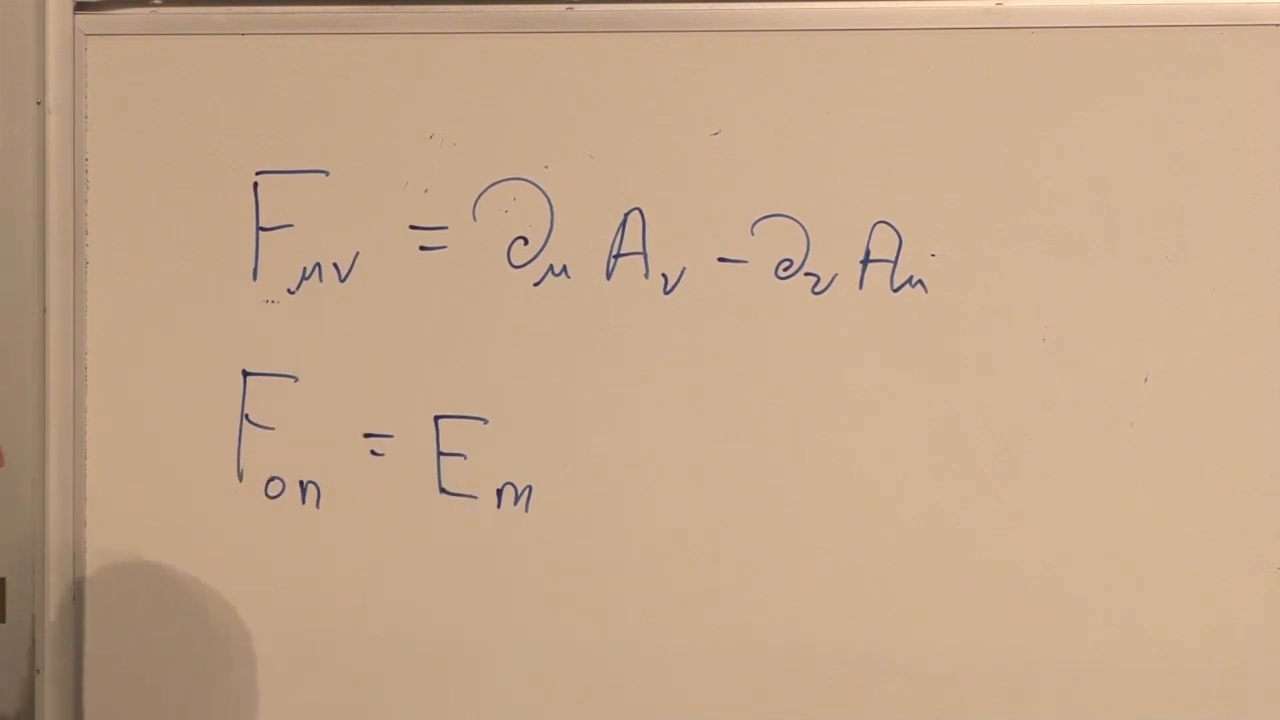
\includegraphics[width=\linewidth]{lecture_08_figure_02.png}\caption{Definition des Feldtensors und seine gemischte Zeit--Raum-Komponente, die mit dem elektrischen Feld identifiziert wird.}\par\smallskip
\textit{Vorlesungsbild: 00:13:15.}\end{figure}

Die Beziehung zum Magnetfeld ist der räumliche Teil derselben Definition. Zum Beispiel gilt
\begin{equation}
B_x
=
\partial_yA_z-\partial_zA_y
=
F_{yz},
\end{equation}
Die beiden anderen Komponenten erhält man durch zyklische Vertauschung.

\begin{figure}[H]\centering
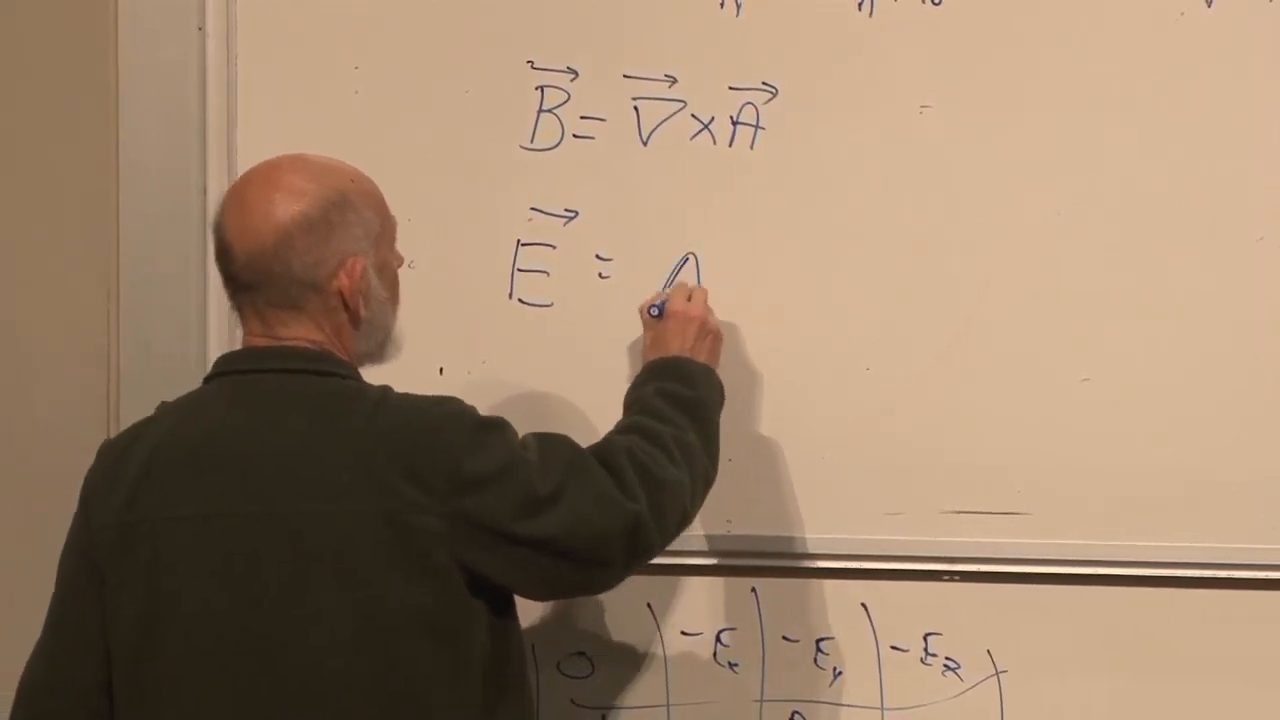
\includegraphics[width=\linewidth]{lecture_08_figure_03.png}\caption{Die Formeln für das elektrische Feld und die Rotation des Vektorpotentials an der Tafel.}\par\smallskip
\textit{Vorlesungsbild: 00:14:00.}\end{figure}

\subsection{Die Komponentenmatrix}

Der erste Tensorindex kennzeichne die Zeilen, der zweite die Spalten, geordnet in der Reihenfolge \(0,x,y,z\). Dann gilt
\begin{equation}
F_{\mu\nu}
=
\begin{pmatrix}
0&E_x&E_y&E_z\\
-E_x&0&B_z&-B_y\\
-E_y&-B_z&0&B_x\\
-E_z&B_y&-B_x&0
\end{pmatrix}.
\label{eq:f-lower-matrix}
\end{equation}
Die gemischte Zeit--Raum-Randkomponente enthält \(\mathbf E\); der räumliche \(3\times3\)-Block enthält \(\mathbf B\). Das untere Dreieck enthält keine neuen Informationen, denn es ist das negative Spiegelbild des oberen Dreiecks.

\begin{figure}[H]\centering
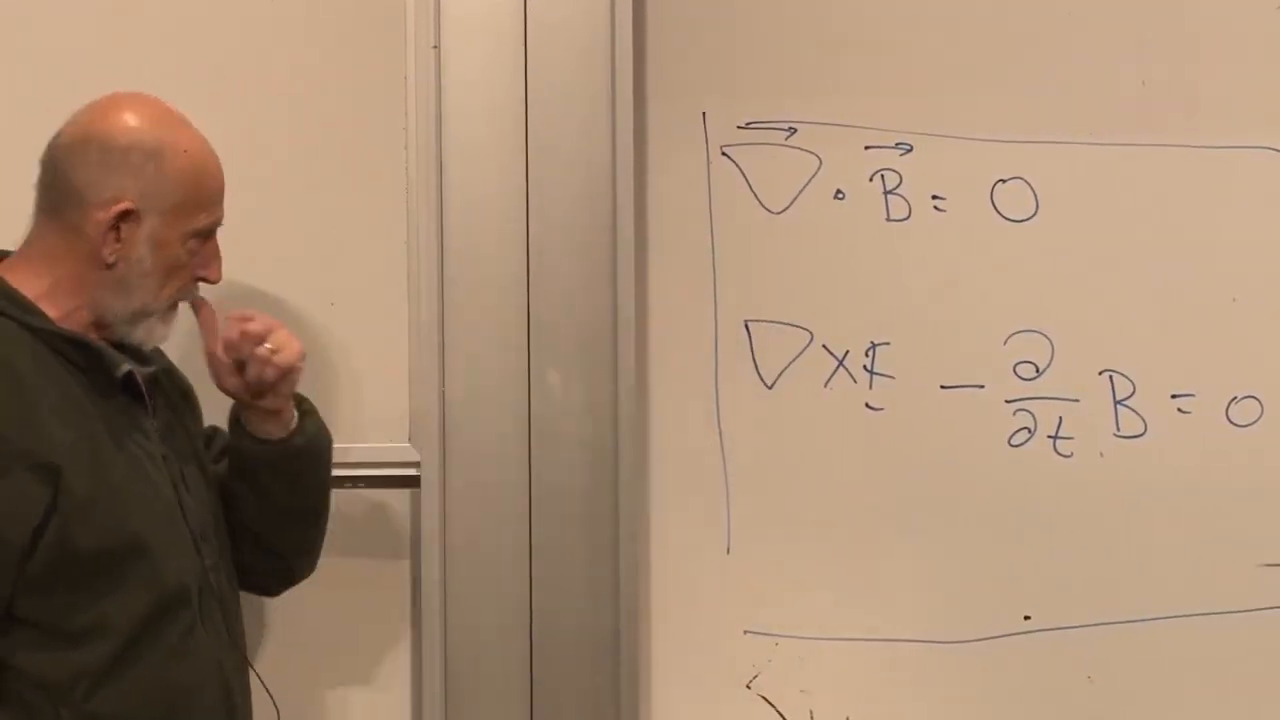
\includegraphics[width=\linewidth]{lecture_08_figure_04.png}\caption{Der vollständig angegebene elektromagnetische Tensor mit unteren Indizes, seinem elektrischen Rand und dem magnetischen räumlichen Block.}\par\smallskip
\textit{Vorlesungsbild: 00:17:15.}\end{figure}

Wenn beide Indizes angehoben werden, ändert sich das Vorzeichen jedes elektrischen Eintrags; die magnetischen Einträge bleiben unverändert:
\begin{equation}
F^{\mu\nu}
=
\begin{pmatrix}
0&-E_x&-E_y&-E_z\\
E_x&0&B_z&-B_y\\
E_y&-B_z&0&B_x\\
E_z&B_y&-B_x&0
\end{pmatrix}.
\label{eq:f-upper-matrix}
\end{equation}
Eine elektrische Komponente enthält einen Zeitindex und erhält daher ein Minuszeichen. Eine magnetische Komponente enthält zwei räumliche Indizes und erhält keines.

\begin{classroomqa}\audiencequestion{Verstehe ich die Matrix richtig: Die magnetischen Komponenten haben keinen Zeitindex?}\lecturerresponse{Ja. Sie liegen im rein räumlichen Block. Die elektrischen Komponenten sind genau die gemischten Zeit--Raum-Einträge in der ersten Zeile und der ersten Spalte. \lecturetimestamp{00:18:55}}\end{classroomqa}

\section{Boost eines rein magnetischen Feldes}

Betrachten wir einen Boost entlang \(x\) mit \(c=1\):
\begin{align}
t'&=\gamma(t-vx),
&
x'&=\gamma(x-vt),
&
y'&=y,
&
z'&=z,
\end{align}
wobei
\begin{equation}
\gamma=\frac{1}{\sqrt{1-v^2}}.
\end{equation}
In Matrixform lautet er
\begin{equation}
x'^\mu
=
\Lambda^\mu{}_\nu x^\nu,
\qquad
\Lambda^\mu{}_\nu
=
\begin{pmatrix}
\gamma&-\gamma v&0&0\\
-\gamma v&\gamma&0&0\\
0&0&1&0\\
0&0&0&1
\end{pmatrix}.
\label{eq:x-boost}
\end{equation}

\begin{classroomqa}\audiencequestion{Fehlt in der Boostmatrix ein Minuszeichen?}\lecturerresponse{Ja. Die außerdiagonalen Zeit--Raum-Einträge tragen die Minuszeichen, die durch \(t'=\gamma(t-vx)\) und \(x'=\gamma(x-vt)\) erforderlich sind. Die Korrektur erfolgt, bevor die Feldtransformation angewendet wird. \lecturetimestamp{00:23:50}}\end{classroomqa}

\begin{figure}[H]\centering
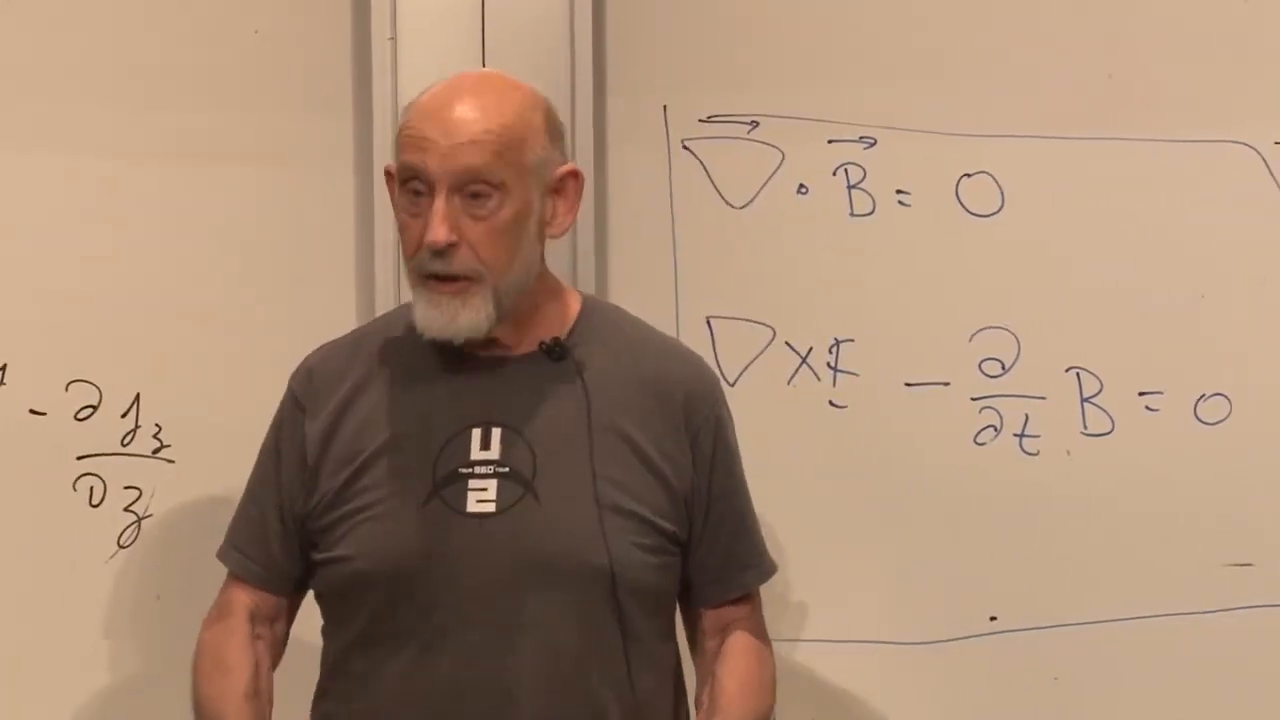
\includegraphics[width=\linewidth]{lecture_08_figure_05.png}\caption{Die korrigierte Lorentz-Boostmatrix für eine Bewegung entlang der \(x\)-Achse.}\par\smallskip
\textit{Vorlesungsbild: 00:24:00.}\end{figure}

Jeder obere Tensorindex transformiert sich wie ein oberer Vektorindex. Daher gilt
\begin{equation}
F'^{\mu\nu}
=
\Lambda^\mu{}_\sigma
\Lambda^\nu{}_\tau
F^{\sigma\tau}.
\label{eq:f-boost-law}
\end{equation}
Die wiederholten Indizes \(\sigma\) und \(\tau\) sind stumme Indizes. Bei einem Tensor mit mehr Indizes tritt für jeden Index eine Transformationsmatrix auf.

\begin{figure}[H]\centering
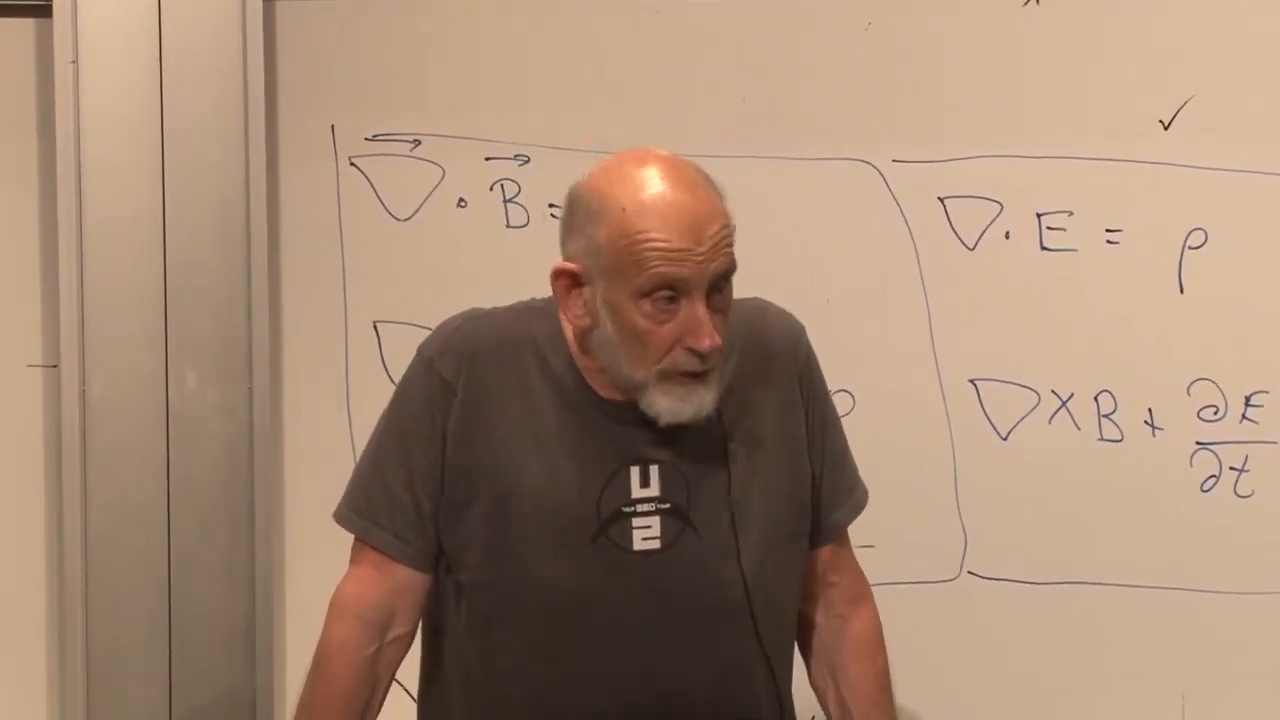
\includegraphics[width=\linewidth]{lecture_08_figure_06.png}\caption{Das Transformationsgesetz für einen Tensor zweiten Ranges unter Lorentz-Transformationen, mit einer Boostmatrix für jeden Index des Feldtensors.}\par\smallskip
\textit{Vorlesungsbild: 00:26:40.}\end{figure}

\subsection{Die Komponente, die elektrisch wird}

Nehmen wir an, das ungestrichene Bezugssystem enthalte nur ein Magnetfeld \(B_y\). Gemäß den Konventionen in Gleichung~\eqref{eq:f-upper-matrix} lautet die relevante unabhängige Komponente
\begin{equation}
F^{xz}=-B_y.
\end{equation}
Gesucht ist die gemischte gestrichene Komponente \(F'^{0z}\), denn sie enthält die gestrichene elektrische Komponente in \(z\)-Richtung. Aus Gleichung
\eqref{eq:f-boost-law} folgt
\begin{align}
F'^{0z}
&=
\Lambda^0{}_\sigma
\Lambda^z{}_\tau F^{\sigma\tau}
\\
&=
\Lambda^0{}_x\Lambda^z{}_zF^{xz}
\\
&=
(-\gamma v)(1)(-B_y)
=
\gamma vB_y.
\end{align}
Da gemäß dieser Konvention \(F'^{0z}=-E'_z\) gilt,
\begin{equation}
E'_z=-\gamma vB_y.
\label{eq:boosted-electric-field}
\end{equation}
Das Vorzeichen hängt von den festgelegten Achsen- und Feldkonventionen ab; der invariante Kern der Rechnung ist
\begin{equation}
\lvert E'_z\rvert
=
\gamma\lvert vB_y\rvert
\ne0.
\end{equation}
Die Doppelsumme reduziert sich darauf, weil das ursprüngliche Feld nur diese eine unabhängige magnetische Komponente besitzt.

\begin{figure}[H]\centering
\includegraphics[width=\linewidth]{lecture_08_figure_07.png}\caption{Die ausgewählte Tensor-Komponente nach dem Boost, mit dem Faktor \(\gamma v\) vor der ursprünglichen magnetischen Komponente.}\par\smallskip
\textit{Vorlesungsbild: 00:32:30.}\end{figure}

Wählen wir das gestrichene Bezugssystem so, dass es sich mit der Ladung bewegt. Dann ruht die Ladung, also gibt es keinen magnetischen Anteil \(q\,\mathbf v'\times\mathbf B'\) ihrer Kraft. Die Kraft verschwindet jedoch nicht: Sie ist \(q\mathbf E'\). Die magnetische Kraft, die der Laborbeobachter beschreibt, und die elektrische Kraft, die der mitbewegte Beobachter beschreibt, sind zwei Beschreibungen desselben Ereignisses.

Damit ist das Rätsel aus Einsteins erstem Absatz gelöst. Die Frage nahm ungefähr die ersten vierzig Minuten dieser Vorlesung ein; der historische Witz dabei ist, dass sie Einstein noch viel länger beschäftigte. Die Rechnung lohnt sich, denn sie macht aus der Aussage, dass sich elektrische und magnetische Felder mischen, eine explizite Tensor-Komponente.

\section{Maxwell-Gleichungen: Identitäten und Dynamik}

Wenden wir uns nun von der Kraft auf eine Ladung den Feldgleichungen zu. In der nächsten Vorlesung werden sie aus einer Wirkung hergeleitet. Hier geht es zunächst darum, sie anzugeben, ihre beiden unterschiedlichen logischen Rollen zu verstehen und den auf Identitäten beruhenden Teil kovariant zu formulieren.

\begin{classroomqa}\audiencequestion{Haben wir diese Gleichungen nicht schon hergeleitet?}\lecturerresponse{Hergeleitet haben wir die Bewegungsgleichung eines geladenen Teilchens in einem vorgegebenen elektromagnetischen Feld. Die Maxwell-Gleichungen sind Bewegungsgleichungen für das Feld selbst, einschließlich seiner Reaktion auf Ladung und Strom. \lecturetimestamp{00:35:10}}\end{classroomqa}

\begin{classroomqa}\audiencequestion{Wie viele Maxwell-Gleichungen gibt es?}\lecturerresponse{Es gibt acht skalare Komponentengleichungen. In Vektorschreibweise fasst man sie als zwei skalare Gleichungen und zwei Vektorgleichungen mit jeweils drei Komponenten zusammen, die man herkömmlich als vier Maxwell-Gleichungen bezeichnet.
\lecturetimestamp{00:35:24}}\end{classroomqa}

Wir verwenden weiterhin Einheiten, in denen \(c=1\) gilt und die üblichen Vakuumkonstanten in die Definitionen von Ladung und Strom aufgenommen wurden. Vier der acht Komponentengleichungen folgen aus der Definition \(F=dA\). Es handelt sich um kinematische Identitäten. Die anderen vier sind dynamisch und könnten sich ändern, wenn sich die Feldwirkung änderte.

\subsection{Drei elementare Vektoroperationen}

Für ein differenzierbares dreidimensionales Vektorfeld \(\mathbf A\) gilt
\begin{align}
(\boldsymbol\nabla\times\mathbf A)_x
&=
\partial_yA_z-\partial_zA_y,
\\
\boldsymbol\nabla\cdot\mathbf A
&=
\partial_xA_x+\partial_yA_y+\partial_zA_z.
\end{align}
Die übrigen Komponenten der Rotation erhält man durch zyklische Vertauschung von \(x\to y\to z\to x\). Für ein skalares Feld \(s\) gilt
\begin{equation}
\boldsymbol\nabla s
=
(\partial_xs,\partial_ys,\partial_zs).
\end{equation}
Die Rotation ist also ein Vektor, die Divergenz ein Skalar und der Gradient ein Vektor.

\begin{classroomqa}\audiencequestion{Muss jemand die Definitionen von Rotation und Divergenz ausführlich wiederholen?}\lecturerresponse{Die Komponentendefinitionen stehen an der Tafel; die übrigen Komponenten müssen nicht alle ausgeschrieben werden. Durch zyklisches Vertauschen der Koordinaten erhält man sie. \lecturetimestamp{00:37:32}}\end{classroomqa}

Aus der Vertauschbarkeit glatter partieller Ableitungen folgen zwei Identitäten:
\begin{align}
\boldsymbol\nabla\cdot
(\boldsymbol\nabla\times\mathbf A)
&=0,
\label{eq:div-curl}
\\
\boldsymbol\nabla\times
(\boldsymbol\nabla s)
&=\mathbf0.
\label{eq:curl-grad}
\end{align}

\begin{classroomqa}\audiencequestion{Sollen wir den vollständigen Komponentenbeweis dafür aufschreiben, dass die Divergenz einer Rotation verschwindet?}\lecturerresponse{Die Klasse verzichtet darauf. Beim Ausmultiplizieren treten Paare wie \(\partial_x\partial_yA_z\) und \(-\partial_y\partial_xA_z\) auf, die sich aufheben, weil sich die Reihenfolge der Ableitungen vertauschen lässt. \lecturetimestamp{00:40:13}}\end{classroomqa}

\begin{figure}[H]\centering
\includegraphics[width=\linewidth]{lecture_08_figure_08.png}\caption{Die Identitäten Divergenz einer Rotation und Rotation eines Gradienten, mit denen sich die eine Hälfte der Maxwell-Gleichungen herleiten lässt.}\par\smallskip
\textit{Vorlesungsbild: 00:41:40.}\end{figure}

\subsection{Keine magnetische Quelle aus dem Vektorpotential}

Bilden wir die Divergenz von Gleichung~\eqref{eq:b-from-a}, so folgt
\begin{equation}
\boldsymbol\nabla\cdot\mathbf B
=
\boldsymbol\nabla\cdot
(\boldsymbol\nabla\times\mathbf A)
=0.
\label{eq:div-b-zero}
\end{equation}
Dabei wurde keine Bewegungsgleichung verwendet. Das Ergebnis folgt allein aus der Potentialbeschreibung und der Vertauschbarkeit glatter Ableitungen.

\begin{figure}[H]\centering
\includegraphics[width=\linewidth]{lecture_08_figure_09.png}\caption{Die Divergenz des Magnetfelds, reduziert auf die Divergenz einer Rotation.}\par\smallskip
\textit{Vorlesungsbild: 00:43:05.}\end{figure}

\begin{classroomqa}\audiencequestion{Was ist die Divergenz des elektrischen Feldes?}\lecturerresponse{In den verwendeten Einheiten ist sie die elektrische Ladungsdichte, \(\boldsymbol\nabla\cdot\mathbf E=\rho\). Eine Punktladung ist das Musterbeispiel für elektrische Feldlinien, die sich von einer Quelle ausbreiten.
\lecturetimestamp{00:43:20}}\end{classroomqa}

Auf elementarer Ebene besagt Gleichung~\eqref{eq:div-b-zero}, dass es keine magnetische Ladungsdichte gibt. Ein glattes, global definiertes Vektorpotential kann keine magnetische Monopolquelle hervorbringen. Diese Aussage muss später eingeschränkt werden: Monopole lassen sich mit Potentialen beschreiben, die auf überlappenden Gebieten definiert sind, oder mit singulären Eichungen. Die Vorlesung verschiebt diese Präzisierung auf später.

\subsection{Die Faraday-Gleichung aus dem elektrischen Potential}

Gleichung~\eqref{eq:e-from-a} lautet in dreidimensionaler Vektorschreibweise
\begin{equation}
\mathbf E
=
\frac{\partial\mathbf A}{\partial t}
-\boldsymbol\nabla A_0.
\label{eq:e-vector-potential}
\end{equation}
Obwohl \(A_0\) zu einem Vierervektor gehört, ist es unter gewöhnlichen räumlichen Drehungen ein Skalar. Bilden wir die Rotation:
\begin{align}
\boldsymbol\nabla\times\mathbf E
&=
\boldsymbol\nabla\times
\frac{\partial\mathbf A}{\partial t}
-
\boldsymbol\nabla\times
(\boldsymbol\nabla A_0)
\\
&=
\frac{\partial}{\partial t}
(\boldsymbol\nabla\times\mathbf A)
\\
&=
\frac{\partial\mathbf B}{\partial t}.
\end{align}
Die räumliche Rotation vertauscht mit der Zeitableitung, während die Rotation des Gradienten verschwindet.

\begin{figure}[H]\centering
\includegraphics[width=\linewidth]{lecture_08_figure_10.png}\caption{Die Rotation des Magnetfelds, die Formel des elektrischen Feldes mit dem Potential und der Beginn der Rotationsrechnung in einem fertigen Tafelbild.}\par\smallskip
\textit{Vorlesungsbild: 00:47:45.}\end{figure}

Die vier homogenen Komponentengleichungen lauten somit
\begin{align}
\boldsymbol\nabla\cdot\mathbf B&=0,
\label{eq:homogeneous-div}
\\
\boldsymbol\nabla\times\mathbf E
-\frac{\partial\mathbf B}{\partial t}
&=\mathbf0.
\label{eq:homogeneous-curl}
\end{align}
Die erste ist eine skalare Gleichung, die zweite eine Vektorgleichung mit drei Komponenten.

\begin{figure}[H]\centering
\includegraphics[width=\linewidth]{lecture_08_figure_11.png}\caption{Das quellenfreie Maxwell-Paar, direkt aus den Potentialdefinitionen erhalten.}\par\smallskip
\textit{Vorlesungsbild: 00:48:45.}\end{figure}

\subsection{Der dynamische Teil}

Die übrigen Gleichungen lauten
\begin{align}
\boldsymbol\nabla\cdot\mathbf E&=\rho,
\label{eq:gauss-electric}
\\
\boldsymbol\nabla\times\mathbf B
+\frac{\partial\mathbf E}{\partial t}
&=-\mathbf J.
\label{eq:ampere-maxwell}
\end{align}
Sie folgen nicht aus \(F=dA\). Sie beschreiben, wie Quellen das Feld erzeugen und verändern; in der nächsten Vorlesung werden sie aus der elektromagnetischen Wirkung hergeleitet. Das Minuszeichen vor dem Strom ergibt sich aus den bereits gewählten Konventionen: \(F_{0i}=E_i\), \(F_{ij}=\epsilon_{ijk}B_k\) und \(\partial_\mu F^{\mu\nu}=J^\nu\). An der Tafel steht zunächst \(\mathbf J\) ohne dieses Minuszeichen auf der rechten Seite; die daraus folgende Unvereinbarkeit mit der Ladungserhaltung wird in der nächsten Vorlesung bemerkt und korrigiert.

\begin{classroomqa}\audiencequestion{Welche Art von Größe steht auf der rechten Seite der Rotationsgleichung?}\lecturerresponse{Die linke Seite ist ein dreidimensionaler Vektor, also ist auch die rechte Seite ein dreidimensionaler Vektor, die elektrische Stromdichte \(\mathbf J\). Auf der rechten Seite der Gauß-Gleichung steht die dreidimensionale skalare Ladungsdichte \(\rho\).
\lecturetimestamp{00:50:36}}\end{classroomqa}

\begin{figure}[H]\centering
\includegraphics[width=\linewidth]{lecture_08_figure_12.png}\caption{Die vier Maxwell-Gleichungen, gruppiert in das auf Identitäten beruhende Paar und das dynamische Paar mit Quellen.}\par\smallskip
\textit{Vorlesungsbild: 00:50:40.}\end{figure}

\section{Ladung und Strom als Raumzeitfluss}

Den Größen \(\rho\) und \(\mathbf J\) müssen nun geometrische Bedeutungen zugewiesen werden. Die Ladungsdichte ist Ladung pro Volumeneinheit; die Stromdichte ist die Ladung, die pro Zeiteinheit eine orientierte Fläche durchquert. Die Vorlesung entwickelt beide Größen aus Weltlinien, damit ihre spätere Zusammenfassung zu einem Vierervektor nicht zufällig erscheint.

\subsection{Eine Randbemerkung aus dem benachbarten Hörsaal}

Bevor wir diese Weltlinien zeichnen, geben Gleichungen, die an der Tafel im Nachbarraum zu sehen sind, Anlass zu einer kurzen didaktischen Randbemerkung. In einem bevorstehenden Kurs sollte Mathematikdozenten Quantenmechanik vermittelt werden, damit sie die nötigen Vorkenntnisse für die Quantenfeldtheorie und deren Verbindungen zur modernen Mathematik erwerben konnten. Die Herausforderung wirkt in beide Richtungen: Der Physiker muss unausgesprochene physikalische Denkweisen explizit machen, während der Mathematiker verstehen muss, was die formalen Strukturen beschreiben sollen.

\begin{classroomqa}\audiencequestion{Wer dürfte diesen Lehrauftrag als frustrierend empfinden?}\lecturerresponse{Möglicherweise beide Seiten: Physiker, die vor einem unvertrauten Publikum lehren, und Mathematiker, die sich mit den physikalischen Denkweisen hinter dem Formalismus auseinandersetzen. Dennoch dürfte der Lehrauftrag Spaß machen. Dann kehrt die Klasse zu Ladung und Strom zurück. \lecturetimestamp{00:53:20}}\end{classroomqa}

\subsection{Ladungsdichte}

Zeichnen wir die Zeit senkrecht und fassen die übrigen gezeichneten Richtungen als dreidimensionalen Raum auf. Geladene Teilchen beschreiben Weltlinien. Wählen wir zu einem festen Zeitpunkt einen kleinen räumlichen Würfel mit Volumen \(\Delta V\), der die Gesamtheit dieser Weltlinien durchschneidet, und addieren wir die Ladungen der Teilchen darin. Die Ladungsdichte ist dann
\begin{equation}
\rho(t,\mathbf x)
=
\lim_{\Delta V\to0}
\frac{\Delta Q}{\Delta V}.
\label{eq:charge-density}
\end{equation}
Das zweidimensionale Quadrat an der Tafel stellt einen dreidimensionalen Würfel dar; die fehlende räumliche Richtung wird nur deshalb nicht gezeichnet, weil sich vier Dimensionen nicht auf einer flachen Tafel darstellen lassen.

\begin{figure}[H]\centering
\includegraphics[width=\linewidth]{lecture_08_figure_13.png}\caption{Weltlinien geladener Teilchen, die eine kleine räumliche Zelle durchqueren, mit \(\rho=\Delta Q/\Delta V\).}\par\smallskip
\textit{Vorlesungsbild: 00:57:20.}\end{figure}

\subsection{Stromdichte}

Drehen wir die Raumzeitzelle auf die Seite. Um \(J_x\) zu definieren, wählen wir ein kleines Fenster mit der Fläche \(\Delta A_x\) in der \(yz\)-Ebene, senkrecht zur \(x\)-Achse. Wir zählen die Nettoladung, die während \(\Delta t\) von der negativen \(x\)-Seite zur positiven \(x\)-Seite übertritt:
\begin{equation}
J_x
=
\lim_{\Delta A_x,\Delta t\to0}
\frac{\Delta Q_x}{\Delta A_x\,\Delta t}.
\label{eq:jx-window}
\end{equation}
Die Orientierung legt das Vorzeichen fest. Fenster senkrecht zu \(y\) und \(z\) definieren auf dieselbe Weise \(J_y\) und \(J_z\).

Die Zeichnung an der Tafel gerät ins Ringen mit der Darstellung: Ein Fenster in der \(yz\)-Ebene sieht eher wie ein Fenster in der Decke als in der Wand aus. Es gibt schlicht mehr relevante Achsen, als sich gleichzeitig darstellen lassen. Die invariante Definition ist eindeutig, auch wenn die Skizze es nicht ist.

\begin{classroomqa}\audiencequestion{Liegt das Fenster in der Zeichnung an der Decke?}\lecturerresponse{In der Analogie mit dem Raum: ja. Entscheidend ist, dass seine Ebene senkrecht zur Richtung \(x\) steht. Eine Fläche \(yz\) misst den Strom in \(x\)-Richtung, der sie durchquert. \lecturetimestamp{00:59:38}}\end{classroomqa}

\begin{figure}[H]\centering
\includegraphics[width=\linewidth]{lecture_08_figure_14.png}\caption{Ladungsstrom durch ein transversales Fenster, mit \(J_x=\Delta Q/(\Delta A\,\Delta t)\).}\par\smallskip
\textit{Vorlesungsbild: 01:01:40.}\end{figure}

\begin{figure}[H]\centering
\includegraphics[width=\linewidth]{lecture_08_figure_15.png}\caption{Die drei Stromkomponenten, definiert über Ladung, die Fenster senkrecht zu den drei räumlichen Achsen durchquert.}\par\smallskip
\textit{Vorlesungsbild: 01:02:40.}\end{figure}

Die vier Größen sind analog definiert. Ein räumliches Volumen zu einem festen Zeitpunkt ist eine Hyperfläche senkrecht zur Zeitachse, sodass \(\rho\) den Ladungsfluss durch ein zeitnormales Fenster angibt. Die Größen \(J_i\) beschreiben Flüsse durch räumlich normale Fenster.

\begin{classroomqa}\audiencequestion{Sind die vier Zahlen ein Fluss in Zeitrichtung und drei Flüsse in den räumlichen Richtungen?}\lecturerresponse{Genau das ist die hilfreiche Vorstellung. Ein räumliches Volumen ist ein Fenster senkrecht zur Zeitachse; die drei transversalen Flächen sind Fenster senkrecht zu \(x\), \(y\) und \(z\). Diese vier Flüsse gehören zusammen. \lecturetimestamp{01:04:14}}\end{classroomqa}

Das legt den kontravarianten Viererstrom nahe:
\begin{equation}
J^\mu
=
(\rho,J_x,J_y,J_z).
\label{eq:four-current}
\end{equation}

\begin{classroomqa}\audiencequestion{Wo kommt die Metrik ins Spiel, und ist dieser Strom kovariant oder kontravariant?}\lecturerresponse{Wie hier definiert, bilden \(\rho\) und die drei Größen \(J_i\) die Komponenten von \(J^\mu\), einem Vierervektor mit oberen Indizes, also einem kontravarianten Vierervektor. Die Metrik senkt den Index, wenn \(J_\mu\) benötigt wird. Die kovariante Formulierung der Maxwell-Gleichungen wird zeigen, warum die Wahl oberer Indizes naheliegt.
\lecturetimestamp{01:04:48}}\end{classroomqa}

\section{Zwischenspiel in der Pause: Signale nahe einem Schwarzen Loch}

In der angesetzten Pause wenden sich die Fragen einer früheren Diskussion über Schwarze Löcher zu. Diese Abschweifung von der Elektrodynamik ist ein ausführlicher Austausch im Hörsaal und veranschaulicht dieselbe Sorgfalt, mit der Beschreibungen verschiedener Beobachter auseinandergehalten werden.

\begin{classroomqa}\audiencequestion{Wenn ein weit entfernter Beobachter sieht, wie ein hineinfallendes Objekt nahe dem Horizont langsamer wird, müsste das Schwarze Loch dann nicht von allem bedeckt erscheinen, was jemals hineingefallen ist?}\lecturerresponse{In der Schwarzschild-Koordinatenzeit scheint klassischer freier Fall den Horizont asymptotisch zu erreichen. Man kann sich aufeinanderfolgende Materie als immer stärker komprimierte Schichten nahe dem Horizont vorstellen. Beobachtbar verzögert sich das ausgesandte Signal jedoch zunehmend, wird rotverschoben und schwächer. Licht, das lokal mit einer gewöhnlichen Frequenz ausgesandt wird, kommt zunächst als sichtbares Licht, dann als Infrarot-, Mikrowellen- und schließlich als Radiostrahlung an; jedes Photon trägt dabei weniger Energie. Kein realistischer weit entfernter Detektor kann ein helles, eingefrorenes Objekt für immer sehen; es verblasst in der Schwärze.
\lecturetimestamp{01:06:11}}\end{classroomqa}

Die Uhr des hineinfallenden Beobachters und die lokal ausgesandte Taschenlampenstrahlung bleiben für diesen Beobachter gewöhnlich. Die Beschreibung aus der Ferne weicht ab, weil sowohl die Frequenz als auch die Ankunftsrate rotverschoben werden. Bei endlicher Energie und endlicher Bandbreite gibt es effektiv einen letzten noch auflösbaren Teil der Nachricht.

\begin{classroomqa}\audiencequestion{Nähert sich das Objekt asymptotisch dem Ereignishorizont?}\lecturerresponse{Das ist die Beschreibung aus der Ferne in Schwarzschild-Koordinaten. Quantentheoretisch muss man das verblassende Signal außerdem von der Hawking-Strahlung des Schwarzen Lochs unterscheiden. Zu hinreichend späten Zeiten geht das schwache rotverschobene Signal in der Hintergrundstrahlung des Schwarzen Lochs selbst beobachtbar verloren. \lecturetimestamp{01:09:24}}\end{classroomqa}

\begin{classroomqa}\audiencequestion{Was, wenn die Wellenlänge der rotverschobenen Strahlung größer wird als die Skala des beobachtbaren Universums?}\lecturerresponse{Praktisch geht das Signal lange vor Erreichen dieser Grenze verloren. Die Vorlesung gibt als grobe Größenordnung für das Hawking-Bild ungefähr ein typisches Quant pro Lichtdurchquerungszeit an:
\[
t_{\rm cross}\sim\frac{R_s}{c}.
\]
Für ein großes Schwarzes Loch ist diese Strahlung außerordentlich schwach, und ein hinreichend stark rotverschobenes Signal des hineinfallenden Objekts wird lange vor jeder kosmologischen Grenze für die Wellenlänge undetektierbar. \lecturetimestamp{01:09:50}}\end{classroomqa}

\begin{classroomqa}\audiencequestion{Bleibt die Rate von ungefähr einem Quant pro Durchquerungszeit während der gesamten Lebensdauer des Schwarzen Lochs gleich?}\lecturerresponse{Nein. Ein verdampfendes Schwarzschild-Schwarzes-Loch schrumpft, sodass seine Durchquerungszeit kürzer und seine Hawking-Temperatur höher wird. Die Emission beschleunigt sich daher. Die Dimensionsabschätzung anhand des momentanen Radius bleibt nützlich, aber der Radius ist nicht konstant. Entsprechend wird die typische Hawking-Wellenlänge im Verlauf der Verdampfung kürzer. \lecturetimestamp{01:11:42}}\end{classroomqa}

Nach der Pause kehren wir, ohne Jackett, zu \(\rho\) und \(\mathbf J\) zurück.

\section{Lokale Ladungserhaltung}

Es liegt nahe, Ladungserhaltung lediglich so anzugeben:
\begin{equation}
\frac{dQ_{\rm universe}}{dt}=0.
\end{equation}
Diese Aussage ist zu schwach. Ladung könnte aus einem Labor verschwinden und sofort bei Alpha Centauri oder noch weiter entfernt im Coma-Haufen wieder auftauchen, ohne dass sich die Gesamtladung änderte. Ein solches Gesetz hätte kaum experimentelle Aussagekraft.

Die stärkere Aussage ist lokal: Die Ladung in einem Gebiet kann sich nur dadurch ändern, dass Ladung die Grenze dieses Gebiets überquert. Legen wir einen kleinen Kasten um einen Punkt. Nimmt seine Ladung zu, muss durch seine sechs Seitenflächen netto einwärts gerichteter Strom fließen; nimmt sie ab, muss netto Strom nach außen fließen.

\subsection{Fluss durch gegenüberliegende Flächen}

Betrachten wir die beiden Flächen senkrecht zu \(x\). Der Beitrag nach innen auf der einen Fläche wird bei einem bestimmten Wert von \(x\) ausgewertet; der Beitrag auf der gegenüberliegenden Fläche wird bei einem geringfügig entfernten Wert ausgewertet. Ihre Differenz, geteilt durch die Breite des Kastens, geht über in
\begin{equation}
-\partial_xJ_x.
\end{equation}
Das Minuszeichen tritt auf, weil \(J_x\) als Fluss in Richtung zunehmender \(x\) definiert ist, während ein nach außen gerichteter Fluss die Ladung im Kasten verringert. Die Paare der \(y\)- und \(z\)-Flächen tragen entsprechend \(-\partial_yJ_y\) und \(-\partial_zJ_z\) bei. Daher gilt
\begin{equation}
\frac{\partial\rho}{\partial t}
=
-\partial_xJ_x-\partial_yJ_y-\partial_zJ_z
=
-\boldsymbol\nabla\cdot\mathbf J.
\end{equation}
Äquivalent dazu:
\begin{equation}
\boxed{
\frac{\partial\rho}{\partial t}
+\boldsymbol\nabla\cdot\mathbf J=0
}.
\label{eq:continuity}
\end{equation}

\begin{figure}[H]\centering
\includegraphics[width=\linewidth]{lecture_08_figure_16.png}\caption{Das lokale Bilanzgesetz \(\dot\rho=-\boldsymbol\nabla\cdot\mathbf J\) zusammen mit dem kleinen Kasten, dessen Randströme es hervorbringen.}\par\smallskip
\textit{Vorlesungsbild: 01:20:45.}\end{figure}

Dies wird üblicherweise Kontinuitätsgleichung genannt. In der Vorlesung wird die Bezeichnung \emph{lokale Erhaltung} bevorzugt: „Kontinuität“ kann eine mathematische Glattheitsannahme nahelegen, während der physikalische Inhalt darin besteht, dass Ladung nicht hier verschwinden und dort wieder auftauchen kann, ohne dass dazwischen ein Strom fließt.

\subsection{Warum Maxwell den Verschiebungsstrom benötigte}

Gleichung~\eqref{eq:continuity} ist keine unabhängige Ergänzung der Maxwell-Gleichungen. Wir bilden die Zeitableitung des Gaußschen Gesetzes und die Divergenz des Ampère--Maxwell-Gesetzes:
\begin{align}
\frac{\partial\rho}{\partial t}
&=
\boldsymbol\nabla\cdot
\frac{\partial\mathbf E}{\partial t},
\\
-\boldsymbol\nabla\cdot\mathbf J
&=
\boldsymbol\nabla\cdot
(\boldsymbol\nabla\times\mathbf B)
+
\boldsymbol\nabla\cdot
\frac{\partial\mathbf E}{\partial t}
\\
&=
\boldsymbol\nabla\cdot
\frac{\partial\mathbf E}{\partial t}.
\end{align}
Die beiden linken Seiten sind daher gleich, woraus
\(\partial_t\rho=-\boldsymbol\nabla\cdot\mathbf J\) folgt – genau
Gleichung~\eqref{eq:continuity}. Entscheidend ist hier die Struktur: Die Zeitableitung von \(\mathbf E\), der Verschiebungsstromterm, ist wesentlich, damit die Divergenzrelation mit der Ladungserhaltung vereinbar ist.

\begin{classroomqa}
\audiencequestion{Wir haben doch nicht gezeigt, woher die beiden quellenbehafteten Maxwell-Gleichungen kommen, oder?}
\lecturerresponse{Nein. Sie sind das dynamische Ziel und werden nächstes Mal aus der Wirkung hergeleitet. Das magnetostatische Wirbelgesetz war schon vor Maxwell bekannt; Maxwells entscheidende zeitabhängige Ergänzung war der Verschiebungsstrom. Durch ihn ist die Feldgleichung mit der lokalen Ladungserhaltung vereinbar. \lecturetimestamp{01:23:15}}
\end{classroomqa}

Die ausführliche Divergenzrechnung wird in der Vorlesung als Übung überlassen, aber ihre Schlussfolgerung ist zwingend: Die Maxwell-Gleichungen erfordern Ladungserhaltung.

\section{Der Viererstrom und seine Divergenz}

Schreiben wir Gleichung~\eqref{eq:continuity} komponentenweise:
\begin{equation}
\frac{\partial\rho}{\partial t}
+
\frac{\partial J_x}{\partial x}
+
\frac{\partial J_y}{\partial y}
+
\frac{\partial J_z}{\partial z}
=0.
\label{eq:continuity-components}
\end{equation}

\begin{figure}[H]
\centering
\includegraphics[width=\linewidth]{lecture_08_figure_17.png}
\caption{Die lokale Ladungserhaltung, aufgeschlüsselt in eine Zeitableitung und drei räumliche Ableitungen.}
\par\smallskip
\textit{Vorlesungszeit: 01:25:40.}
\end{figure}

Mit \(J^\mu\), definiert durch Gleichung~\eqref{eq:four-current}, lassen sich die vier Terme zu einer Kontraktion zusammenfassen:
\begin{equation}
\boxed{\partial_\mu J^\mu=0}.
\label{eq:four-current-conservation}
\end{equation}
Der untere Index von \(\partial_\mu\) wird mit dem oberen Index von \(J^\mu\) kontrahiert; das Ergebnis ist daher ein Lorentz-Skalar. Die geometrische Konstruktion des Fensters deutete dieses Transformationsgesetz bereits an: \(\rho\) und die drei Stromkomponenten sind vier Orientierungen desselben Ladungsflusses.

\begin{figure}[H]
\centering
\includegraphics[width=\linewidth]{lecture_08_figure_18.png}
\caption{Die Komponenten \((\rho,J_x,J_y,J_z)\) werden zu \(J^\mu\) zusammengesetzt und mit dem Vierergradienten kontrahiert.}
\par\smallskip
\textit{Vorlesungszeit: 01:27:10.}
\end{figure}

\begin{classroomqa}
\audiencequestion{Wann wurde aus der Zeitableitung von \(\rho\) eine partielle Ableitung?}
\lecturerresponse{Sie war von Anfang an eine partielle Ableitung. Wir halten das räumliche Kästchen fest und fragen, wie sich seine Ladungsdichte mit der Zeit verändert. Wir verfolgen keine bewegte Bahn. Daher bedeutet \(\dot\rho\) hier \(\partial\rho/\partial t\) bei festgehaltenem \(x,y,z\).
\lecturetimestamp{01:28:20}}
\end{classroomqa}

\section{Die homogenen Gleichungen in kovarianter Form}

Wir verfügen nun über die benötigten Größen:
\begin{itemize}
\item \(\mathbf E\) und \(\mathbf B\) sind die sechs unabhängigen Komponenten des antisymmetrischen Tensors \(F_{\mu\nu}\);
\item \(\rho\) und \(\mathbf J\) sind die vier Komponenten von \(J^\mu\);
\item die lokale Erhaltung ist die skalare Gleichung
\(\partial_\mu J^\mu=0\).
\end{itemize}
Als verbleibende Aufgabe für diese Vorlesung müssen wir das Paar homogener Maxwell-Gleichungen, Gleichungen~\eqref{eq:homogeneous-div} und
\eqref{eq:homogeneous-curl}, in einer einzigen Tensor-Gleichung zusammenfassen.

\subsection{Die zyklische Ableitung}

Die gesuchte Gleichung lautet
\begin{equation}
\boxed{
\partial_\sigma F_{\nu\tau}
+
\partial_\nu F_{\tau\sigma}
+
\partial_\tau F_{\sigma\nu}
=0
}.
\label{eq:bianchi}
\end{equation}
In den drei Termen werden der Ableitungsindex und die beiden Indizes des Feldtensors zyklisch vertauscht. Oft schreibt man dies abgekürzt als
\begin{equation}
\partial_{[\sigma}F_{\nu\tau]}=0,
\end{equation}
wobei eckige Klammern die Antisymmetrisierung bezeichnen.

\begin{figure}[H]
\centering
\includegraphics[width=\linewidth]{lecture_08_figure_19.png}
\caption{Die zyklische Gleichung mit drei Indizes, die die homogenen Maxwell-Gleichungen zusammenfasst.}
\par\smallskip
\textit{Vorlesungszeit: 01:33:20.}
\end{figure}

\subsection{Alle drei Indizes räumlich}

Setzen wir
\begin{equation}
(\sigma,\nu,\tau)=(x,y,z).
\end{equation}
Dann gilt
\begin{align}
0
&=
\partial_xF_{yz}
+
\partial_yF_{zx}
+
\partial_zF_{xy}
\\
&=
\partial_xB_x+\partial_yB_y+\partial_zB_z
\\
&=
\boldsymbol\nabla\cdot\mathbf B.
\end{align}
Die Komponente von Gleichung~\eqref{eq:bianchi}, bei der alle Indizes räumlich sind, besagt somit genau, dass die magnetische Divergenz verschwindet.

\begin{figure}[H]
\centering
\includegraphics[width=\linewidth]{lecture_08_figure_20.png}
\caption{Die Komponente der zyklischen Identität mit ausschließlich räumlichen Indizes reduziert sich auf \(\partial_xB_x+\partial_yB_y+\partial_zB_z=0\).}
\par\smallskip
\textit{Vorlesungszeit: 01:35:30.}
\end{figure}

\subsection{Ein Zeitindex}

Wählen wir beispielsweise
\begin{equation}
(\sigma,\nu,\tau)=(y,x,0).
\end{equation}
Dann verbindet Gleichung~\eqref{eq:bianchi} zwei räumliche Ableitungen elektrischer Komponenten mit einer Zeitableitung einer magnetischen Komponente:
\begin{equation}
\partial_yF_{x0}
+
\partial_xF_{0y}
+
\partial_0F_{yx}
=0.
\end{equation}
Mit der Matrix aus Gleichung~\eqref{eq:f-lower-matrix} ist dies eine Komponente von
\begin{equation}
\boldsymbol\nabla\times\mathbf E
-\frac{\partial\mathbf B}{\partial t}
=\mathbf0,
\end{equation}
wobei die relativen Vorzeichen durch die Antisymmetrie festgelegt sind. Die Wahl der anderen Paare räumlicher Indizes liefert die beiden übrigen Komponenten der Rotation.

\begin{figure}[H]
\centering
\includegraphics[width=\linewidth]{lecture_08_figure_21.png}
\caption{Eine Prüfung mit einem Zeitindex und zwei Raumindizes ergibt eine Komponente der Faraday-Gleichung.}
\par\smallskip
\textit{Vorlesungszeit: 01:38:20.}
\end{figure}

Es gibt auch einen direkten Beweis. Setzen wir Gleichung~\eqref{eq:field-tensor-definition} in Gleichung~\eqref{eq:bianchi} ein. Dabei entstehen sechs Terme mit zweiten Ableitungen, die sich paarweise aufheben, weil partielle Ableitungen vertauschbar sind. Dies ist die vierdimensionale Version der Identitäten für die Divergenz einer Rotation und die Rotation eines Gradienten.

\begin{classroomqa}
\audiencequestion{Kommt im Namen Bianchi ein \(h\) vor?}
\lecturerresponse{Ja. Die zyklische Gleichung ist die elektromagnetische Bianchi-Identität, ein Spezialfall einer geometrischen Identität, die auch in der allgemeinen Relativitätstheorie auftritt. Ihre tiefere geometrische Deutung wird später behandelt.
\lecturetimestamp{01:40:28}}
\end{classroomqa}

\subsection{Warum vierundsechzig hingeschriebene Komponenten nur vier Gleichungen enthalten}

Drei Indizes mit jeweils vier möglichen Werten scheinen \(4^3=64\) Gleichungen zu ergeben. Die Antisymmetrie beseitigt die Redundanz:
\begin{itemize}
\item Wenn zwei Indizes übereinstimmen, verschwindet der zyklische Ausdruck identisch;
\item Sind alle drei Indizes verschieden, ergeben Permutationen bis auf ein Vorzeichen dieselbe Gleichung;
\item In vier Dimensionen gibt es nur \(\binom{4}{3}=4\) ungeordnete Tripel verschiedener Indizes.
\end{itemize}
Es gibt \(24\) geordnete Tripel mit lauter verschiedenen Indizes; sie gruppieren sich in vier Mengen aus jeweils sechs Permutationen. Die übrigen \(40\) geordneten Tripel verschwinden. Die vier unabhängigen Gleichungen bestehen aus einer Gleichung für die magnetische Divergenz und den drei Komponenten der Faraday-Gleichung.

\begin{classroomqa}
\audiencequestion{Der Feldtensor hat sechs unabhängige Einträge, aber der Ausdruck mit drei Indizes scheint vierundsechzig Gleichungen zu enthalten. Warum bleiben nur vier übrig?}
\lecturerresponse{Bei wiederholten Indizes ergibt sich null; Permutationen dreier verschiedener Indizes wiederholen dieselbe Relation bis auf ein Vorzeichen. Die scheinbar vierundsechzig Komponenten reduzieren sich daher auf vier unabhängige Gleichungen.
\lecturetimestamp{01:41:58}}
\end{classroomqa}

Gleichung~\eqref{eq:bianchi} ist offensichtlich tensorial und damit Lorentz-kovariant. In der glatten Beschreibung mit einem einzigen Potential besagt sie außerdem, dass es weder eine magnetische Ladungsdichte noch einen magnetischen Strom gibt. Das dynamische, quellenbehaftete Gleichungspaar bleibt genau an dem Punkt, den die Vorlesung erreicht hat: Seine kovariante Gleichung und ihre Herleitung aus der Wirkung folgen in der nächsten Sitzung.

\section{Dualität und die Frage nach dem Monopol}

Die abschließenden Fragen greifen die scheinbare Asymmetrie zwischen elektrischen und magnetischen Quellen wieder auf. Im leeren Raum besitzen die Maxwell-Gleichungen eine elektrische--magnetische Dualitätsdrehung:
\begin{equation}
\mathbf E\longrightarrow\mathbf B,
\qquad
\mathbf B\longrightarrow-\mathbf E.
\label{eq:duality-quarter-turn}
\end{equation}
Dies ist eine Drehung um neunzig Grad in einer abstrakten Ebene mit den Achsen \(\mathbf E\) und \(\mathbf B\), keine Spiegelung, die lediglich ihre Bezeichnungen vertauscht. Sind sowohl elektrische als auch magnetische Quellen vorhanden, müssen sich die elektrischen und magnetischen Viererströme gleichzeitig mitdrehen.

\begin{figure}[H]
\centering
\includegraphics[width=\linewidth]{lecture_08_figure_22.png}
\caption{Die abschließende elektrische--magnetische Dualitätsdarstellung: eine Vierteldrehung in der \(E\)-\(B\)-Ebene statt einer bloßen Vertauschung.}
\par\smallskip
\textit{Vorlesungszeit: 01:45:00.}
\end{figure}

\begin{classroomqa}
\audiencequestion{Wenn die quellenfreien Gleichungen unter der Vertauschung von elektrisch und magnetisch dual sind, warum sind dann die elektrischen Komponenten Zeit--Raum-Einträge, während die magnetischen Komponenten Raum--Raum-Einträge sind?}
\lecturerresponse{Die Unterscheidung hängt innerhalb von \(F_{\mu\nu}\) vom Bezugssystem ab, und die quellenfreien Gleichungen lassen eine Dualitätsdrehung zu. Die richtige Operation ist \(\mathbf E\to\mathbf B\) und \(\mathbf B\to-\mathbf E\); werden magnetische Ladungen berücksichtigt, müssen sich die Quellenströme entsprechend mitdrehen. Eine bloße Vertauschung lässt das erforderliche Vorzeichen außer Acht. \lecturetimestamp{01:43:25}}
\end{classroomqa}

\begin{classroomqa}
\audiencequestion{Macht die klare Tensorbeschreibung einen magnetischen Monopol bedeutungslos?}
\lecturerresponse{Nein. Sie bedeutet, dass sich ein Monopol nicht mit einem einzigen glatten Vektorpotential im gesamten Raum darstellen lässt. Stattdessen muss das Potential stückweise definiert, auf eine eichabhängige Weise singulär gemacht oder durch eine äquivalente duale Beschreibung ersetzt werden. Ein elementarer magnetischer Monopol war nicht beobachtet worden, und die Vorlesung kündigt an, später darauf zurückzukommen, wie Monopole in den Formalismus passen, statt die Frage am Ende des Abends zu erzwingen.
\lecturetimestamp{01:45:50}}
\end{classroomqa}

Die Vorlesung endet damit an einer klar bestimmten Grenze. Die Relativitätstheorie hat erklärt, warum sich elektrische und magnetische Felder mischen. Die Definitionen über Potentiale haben die homogenen Maxwell-Gleichungen und ihre Bianchi-Form geliefert. Der Ladungsfluss ist zum Viererstrom geworden, und die lokale Erhaltung hat die Form \(\partial_\mu J^\mu=0\) angenommen. Was noch fehlt, ist die Dynamik: die elektromagnetische Wirkung und die kovariante quellenbehaftete Feldgleichung.